\documentclass[../../../analisi-dei-requisiti.tex]{subfiles}

\begin{document}

\begin{figure}[H]
  \centering
  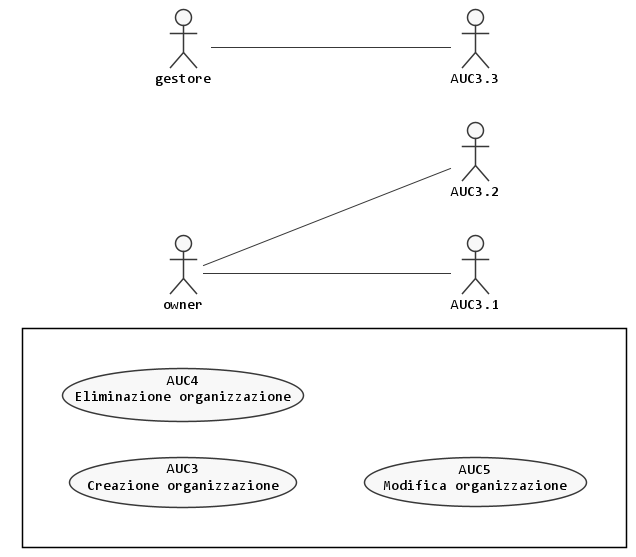
\includegraphics[width=150mm]{gestione-organizzazione.png}
  \caption{AUC3: Gestione organizzazione}%
  \label{fig:AUC3}
\end{figure}

\begin{description}
  \item[Codice:] AUC3;
  \item[Titolo:] Gestione organizzazione;
  \item[Attori primari:] owner;
  \item[Precondizione:] il sistema deve rendere disponibile la pagina di gestione dell'organizzazione;
  \item[Postcondizione:] viene gestita un'organizzazione;
  \item[Scenario principale:]
        \begin{enumerate}
          \item sorge la necessità di effettuare operazioni su un'organizzazione;
        \end{enumerate}
\end{description}

\subsubsection{AUC3.1: Creazione organizzazione}%
\label{subs:AUC3.1}

\begin{figure}[H]
  \centering
  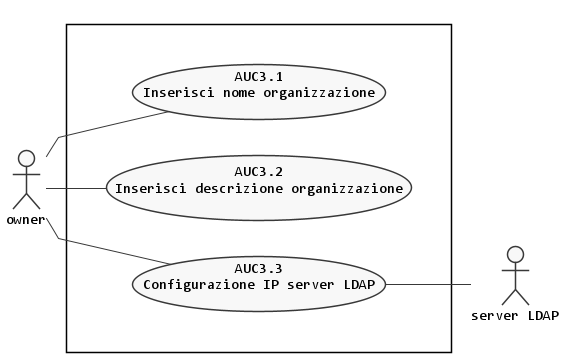
\includegraphics[width=100mm]{creazione-organizzazione.png}
  \caption{AUC3.1: Creazione organizzazione}%
  \label{fig:AUC3_1}
\end{figure}

\begin{description}
  \item[Codice:] AUC3.1;
  \item[Titolo:] Creazione organizzazione;
  \item[Attori primari:] owner;
  \item[Attori secondari:] server LDAP\@;
  \item[Precondizione:] l'organizzazione non deve esistere nella lista di \emph{Stalker};
  \item[Postcondizione:] l'organizzazione viene creata;
  \item[Scenario principale:]
        \begin{enumerate}
          \item sorge la necessità di creare un'organizzazione;
        \end{enumerate}
  \item[Inclusioni:]
        \begin{enumerate}
          \item alla fine della procedura di creazione dell'organizzazione, tutte le applicazioni mobile riceveranno una notifica di aggiornamento
                della lista di organizzazioni~\ref{subs:AUC3.5};
        \end{enumerate}
\end{description}

\subsubsection{AUC3.1.1: Inserisci nome organizzazione}%
\label{subs:AUC3.1.1}
\begin{description}
  \item[Codice:] AUC3.1.1;
  \item[Titolo:] Inserisci nome organizzazione;
  \item[Attori primari:]  owner;
  \item[Precondizione:] il sistema deve rendere disponibile la possibilità di inserire il nome di una nuova organizzazione;
  \item[Postcondizione:] il nome viene opportunamente inserito;
  \item[Scenario principale:]
        \begin{enumerate}
          \item si vuole inserire il nome di un'organizzazione.
        \end{enumerate}

\end{description}

\subsubsection{AUC3.1.2: Inserisci descrizione organizzazione}%
\label{subs:AUC3.1.2}
\begin{description}
  \item[Codice:] AUC3.1.2;
  \item[Titolo:] Inserisci descrizione organizzazione;
  \item[Attori primari:] owner;
  \item[Precondizione:] il sistema deve rendere disponibile la possibilità di inserire una descrizione di una nuova organizzazione;
  \item[Postcondizione:] la descrizione viene opportunamente inserita;
  \item[Scenario principale:]
        \begin{enumerate}
          \item si vuole inserire la descrizione di un'organizzazione.
        \end{enumerate}
\end{description}

\subsubsection{AUC3.1.3: Configurazione dettagli server LDAP}%
\label{subs:AUC3.1.3}
\begin{description}
  \item[Codice:] AUC3.1.3;
  \item[Titolo:] Configurazione dettagli server LDAP\@;
  \item[Attori primari:] owner;
  \item[Attori secondari:] server LDAP\@;
  \item[Precondizione:] il sistema deve rendere disponibile la possibilità di configurazione del server LDAP\@;
  \item[Postcondizione:] il server LDAP è stato configurato;
  \item[Scenario principale:]
        \begin{enumerate}
          \item si vogliono configurare i dettagli del \glossario{server LDAP} che le applicazioni mobile dovranno utilizzare per registrarsi ad un'organizzazione;
          \item se l'organizzazione è segnata come pubblica, i parametri del server LDAP non verranno configurati.
        \end{enumerate}
\end{description}

\subsubsection{AUC3.2: Eliminazione organizzazione}%
\label{subs:AUC3.2}
\begin{description}
  \item[Codice:] AUC3.2;
  \item[Titolo:] Eliminazione organizzazione;
  \item[Attori primari:] owner;
  \item[Precondizione:] deve essere stata selezionata l'organizzazione da eliminare, presente nella lista di \emph{Stalker};
  \item[Postcondizione:] l'organizzazione viene eliminata;
  \item[Scenario principale:]
        \begin{enumerate}
          \item sorge la necessità di eliminare un'organizzazione;
        \end{enumerate}
  \item[Inclusioni:]
        \begin{enumerate}
          \item viene selezionata un'organizzazione~\ref{subs:AUC3.4};
          \item alla fine della procedura di eliminazione dell'organizzazione, tutte le applicazioni mobile riceveranno una notifica di aggiornamento della lista di organizzazioni~\ref{subs:AUC3.5};
        \end{enumerate}
\end{description}

\begin{figure}[H]
  \centering
  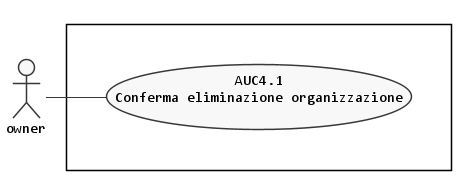
\includegraphics[width=100mm]{eliminazione-organizzazione.png}
  \caption{AUC3.2: Eliminazione organizzazione}%
  \label{fig:AUC3.2}
\end{figure}

\subsubsection{AUC3.2.1: Conferma eliminazione organizzazione}%
\label{subs:AUC3.2.1}
\begin{description}
  \item[Codice:] AUC3.2.1;
  \item[Titolo:] Conferma eliminazione organizzazione;
  \item[Attori primari:] owner;
  \item[Precondizione:] deve essere stata selezionata l'organizzazione da eliminare;
  \item[Postcondizione:] viene confermata l'eliminazione dell'organizzazione;
  \item[Scenario principale:]
        \begin{enumerate}
          \item l'owner visualizza la conferma di eliminazione di un'organizzazione;
        \end{enumerate}
\end{description}

\subsubsection{AUC3.3: Modifica organizzazione}%
\label{subs:AUC3.3}

\begin{figure}[H]
  \centering
  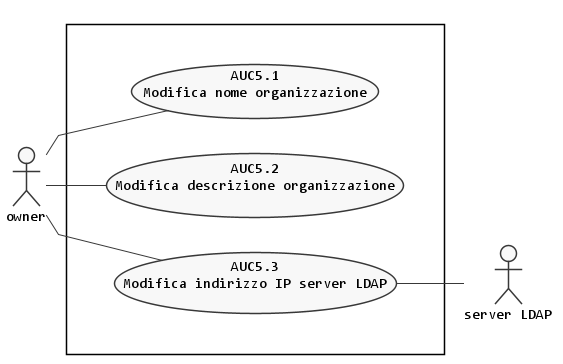
\includegraphics[width=100mm]{modifica-organizzazione.png}
  \caption{AUC3.3: Modifica organizzazione}%
  \label{fig:AUC3_3}
\end{figure}

\begin{description}
  \item[Codice:] AUC3.3;
  \item[Titolo:] Modifica organizzazione;
  \item[Attori primari:] owner;
  \item[Attori secondari:] server LDAP\@;
  \item[Precondizione:] l'owner seleziona l'organizzazione da modificare, presente nella lista di \emph{Stalker};
  \item[Postcondizione:] l'organizzazione viene modificata;
  \item[Scenario principale:]
        \begin{enumerate}
          \item sorge la necessità di modificare un'organizzazione.
        \end{enumerate}
  \item[Inclusioni:]
        \begin{enumerate}
          \item viene scelta un'organizzazione~\ref{subs:AUC3.4}.
        \end{enumerate}
\end{description}

\subsubsection{AUC3.3.1: Modifica nome organizzazione}%
\label{subs:AUC3.3.1}
\begin{description}
  \item[Codice:] AUC3.3.1;
  \item[Titolo:] Modifica nome organizzazione;
  \item[Attori primari:] owner;
  \item[Precondizione:] il sistema deve rendere disponibile la possibilità di modificare il nome di un'organizzazione;
  \item[Postcondizione:] il nome viene opportunamente modificato;
  \item[Scenario principale:]
        \begin{enumerate}
          \item si vuole modificare il nome di un'organizzazione.
        \end{enumerate}
\end{description}

\subsubsection{AUC3.3.2: Modifica descrizione organizzazione}%
\label{subs:AUC3.3.2}
\begin{description}
  \item[Codice:] AUC3.3.2;
  \item[Titolo:] Modifica descrizione organizzazione;
  \item[Attori primari:] owner;
  \item[Precondizione:] il sistema deve rendere disponibile la possibilità di modificare la descrizione di un'organizzazione;
  \item[Postcondizione:] la descrizione viene opportunamente modificata;
  \item[Scenario principale:]
        \begin{enumerate}
          \item si vuole modificare la descrizione di un'organizzazione.
        \end{enumerate}
\end{description}


\subsubsection{AUC3.3.3: Modifica configurazione dettagli server LDAP}%
\label{subs:AUC3.3.3}
\begin{description}
  \item[Codice:] AUC3.3.3;
  \item[Titolo:] Configurazione dettagli server LDAP\@;
  \item[Attori primari:] owner;
  \item[Attori secondari:] server LDAP\@;
  \item[Precondizione:] il sistema deve rendere disponibile la possibilità di modifica configurazione del server LDAP\@;
  \item[Postcondizione:] il server LDAP è stato configurato;
  \item[Scenario principale:]
        \begin{enumerate}
          \item si vuole modificare la configurazione del server LDAP\@.
        \end{enumerate}
\end{description}

\subsubsection{AUC3.4: Seleziona organizzazione}%
\label{subs:AUC3.4}
\begin{description}
  \item[Codice:] AUC3.4;
  \item[Titolo:] Seleziona organizzazione;
  \item[Attori primari:] gestore;
  \item[Precondizione:] il sistema deve mostrare la lista di organizzazioni in \emph{Stalker};
  \item[Postcondizione:] viene scelta l'organizzazione desiderata;
  \item[Scenario principale:]
        \begin{enumerate}
          \item sorge la necessità di effettuare operazioni su un'organizzazione, e viene offerta la possibilità di selezionarla.
        \end{enumerate}
\end{description}

\subsubsection{AUC3.5: Invio richiesta aggiornamento lista organizzazioni}%
\label{subs:AUC3.5}
\begin{description}
  \item[Codice:] AUC3.5;
  \item[Titolo:] Invio richiesta aggiornamento lista organizzazioni;
  \item[Attori primari:] gestore;
  \item[Precondizione:] il sistema mostra la pagina di creazione o eliminazione di un'organizzazione;
  \item[Postcondizione:] la richiesta di aggiornamento della lista delle organizzazioni viene inviata a tutte le applicazioni mobile;
  \item[Scenario principale:]
        \begin{enumerate}
          \item una volta creata o eliminata un'organizzazione, la lista delle organizzazioni viene aggiornata e inviata a tutti gli utenti che hanno installato l'applicazione mobile.
        \end{enumerate}
\end{description}

\end{document}
